\section{\texorpdfstring{\Z}{Z} + fake Background}
\label{sec:bkg_fakeLight}

The \Z + fake process contributes about 17\,\% of the total background. Since the fake leptons are not modeled with sufficient precision by simulation, we employ a data-driven method that uses correlated objects in order to predict the \Z + fake background.


\subsection{Method}
\label{sec:bkg_fakeLight/Method}

To determine the background with fake electrons and muons, we rely on looser objects measured in data that are emitted in a similar way in the decay chain and are therefore expected to be correlated with the fake leptons, and use them as lepton proxies.\footnote{These looser objects are not necessarily leptons as well. For example, a photon that converts into two leptons, one of which has very low \pt, may have kinematics which are very similar to the ones of the other conversion lepton that carries most of the \pt. (Of course, the selection of such objects may be tricky.)} We verify that the kinematic properties of these proxies resemble those of the fake leptons. We then generate a fake sample based on the 2$\ell$+[proxy object] data, treating the proxy objects as leptons (``seed sample''). Further down in the analysis chain, these fake leptons simply appear as regular leptons (\eg when computing invariant masses). Proxy objects that can take multiple roles are considered the appropriate number of times (see below).

The number of 3$\ell$ events in data per 2$\ell$+[proxy object] event in this fake sample is then evaluated (``fake rate''). With the help of the fake rate, we predict the background in the signal regions, by applying it to the corresponding seed sample which requires one less lepton and a proxy object instead. Because the proxy objects appear as leptons, this is simply done by selecting the signal region from the fake sample and multiplying the yield by the fake rate.

To compute the fake rate $\frac{N(3\ell)}{N(2\ell + \textrm{[proxy object])}}$, we subtract contributions from other backgrounds in the numerator and the denominator. This step interacts with the MC background normalizations and thus requires an iterative process to converge. The fake rate then describes the number of fake leptons as a fraction of the number of 2$\ell$+[proxy object] events from all processes that have not been modeled otherwise.

When we apply the fake rate in a signal region, we multiply it by the total number of 2$\ell$+[proxy object] events found in the corresponding seed region in data. However, we use MC to obtain the fake contribution for certain backgrounds.\footnote{This is especially important for \ttbar when a b-tag is not present, since the fake rate is higher in \ttbar events, but there is no obvious way to discern these events from non-\ttbar events in the seed sample.} In these cases, double-counting needs to be mitigated. Therefore, we take the 2$\ell$+[proxy object] component of the background MC sample, apply the same fake rate as for data, and subtract the resulting prediction from the regular data-driven prediction (see \eg Sec.~\ref{sec:bkg_tt} for \ttbar). This is equivalent to keeping the seed sample clean of proxies originating from processes that are modeled otherwise. We therefore verify that the number of tracks be modeled correctly in MC (see Sec.~\ref{sec:bkg_tt/dilepton+track}).

In rare cases due to statistical fluctuations, the subtraction might yield a (small) negative number. If that happens, we replace it by zero, to make sure that the background prediction behaves physically reasonably.\footnote{Another option would be to subtract the MC-fake-seed-driven background from the regular \ttbar MC prediction (again with a lower bound at 0). However, 8\TeV cross-checks have shown that this leads to less accurate results.} For technical details, see Appendix~\ref{app:Software/AnalysisPresenter}.

%We also study to what extent the fake rate depends on other properties of the event (for example the jet composition and spectra), and parameterize the fake rate as necessary. The freedom that we find in determining these parameterizations and kinematic weights is used to assess the systematic uncertainty of the background estimate.

\subsection{Fake Leptons from Asymmetric Internal Photon Conversions (AIC)}
\label{sec:bkg_fakeLight/photons}
We look at the number of events that have 3 light leptons (no $\tau_\textrm{had}$) including an OSSF pair below \Z (\ie $m_{\ell\ell} < 81\GeV$), no b-tags, $\HT < 200\GeV$, and $\MET < 50\GeV$. This is essentially the \Z peak region, except that the dilepton invariant mass is not large enough to fall on the \Z peak, and a third lepton is present.

This region primarily contains events from $\Z \to \ell\ell$ where one of the final state leptons radiates an off-shell photon which decays, or\hairspace---\hairspace{}equivalently\hairspace---\hairspace{}internally converts, asymmetrically to two additional leptons, one of which carries very low \pt and is not reconstructed as an independent object in the detector. The process of emission of an off-shell photon through asymmetric internal conversion (AIC) then yields a single reconstructed lepton in the detector \cite{Gray:2011us}. Since the \pt of the lost lepton is low, the leading three leptons nearly reconstruct the invariant mass of the Z peak. The internal conversion process has an infrared singularity, so the distribution of off-shell photon masses is peaked at very low values. The resulting kinematic distribution in this region of phase space is then very similar to the emission of a real on-shell photon. 

We may therefore form a seed sample with photons as proxies for fake leptons coming from asymmetric internal conversion. All combinations are taken into account, \ie dilepton events with a photon enter the fake sample as four event types (two possible flavors, two possible charges). The photons are required to be within $0.30 \leq \Delta R \leq 0.60$ from another light lepton. This is the characteristic distance for radiated photons of the type considered, as can be seen from Fig.~\ref{fig:fakeLight_AIC_DR}.

\begin{figure}
\begin{center}
	\begin{subfigure}[b]{.7\textwidth}
		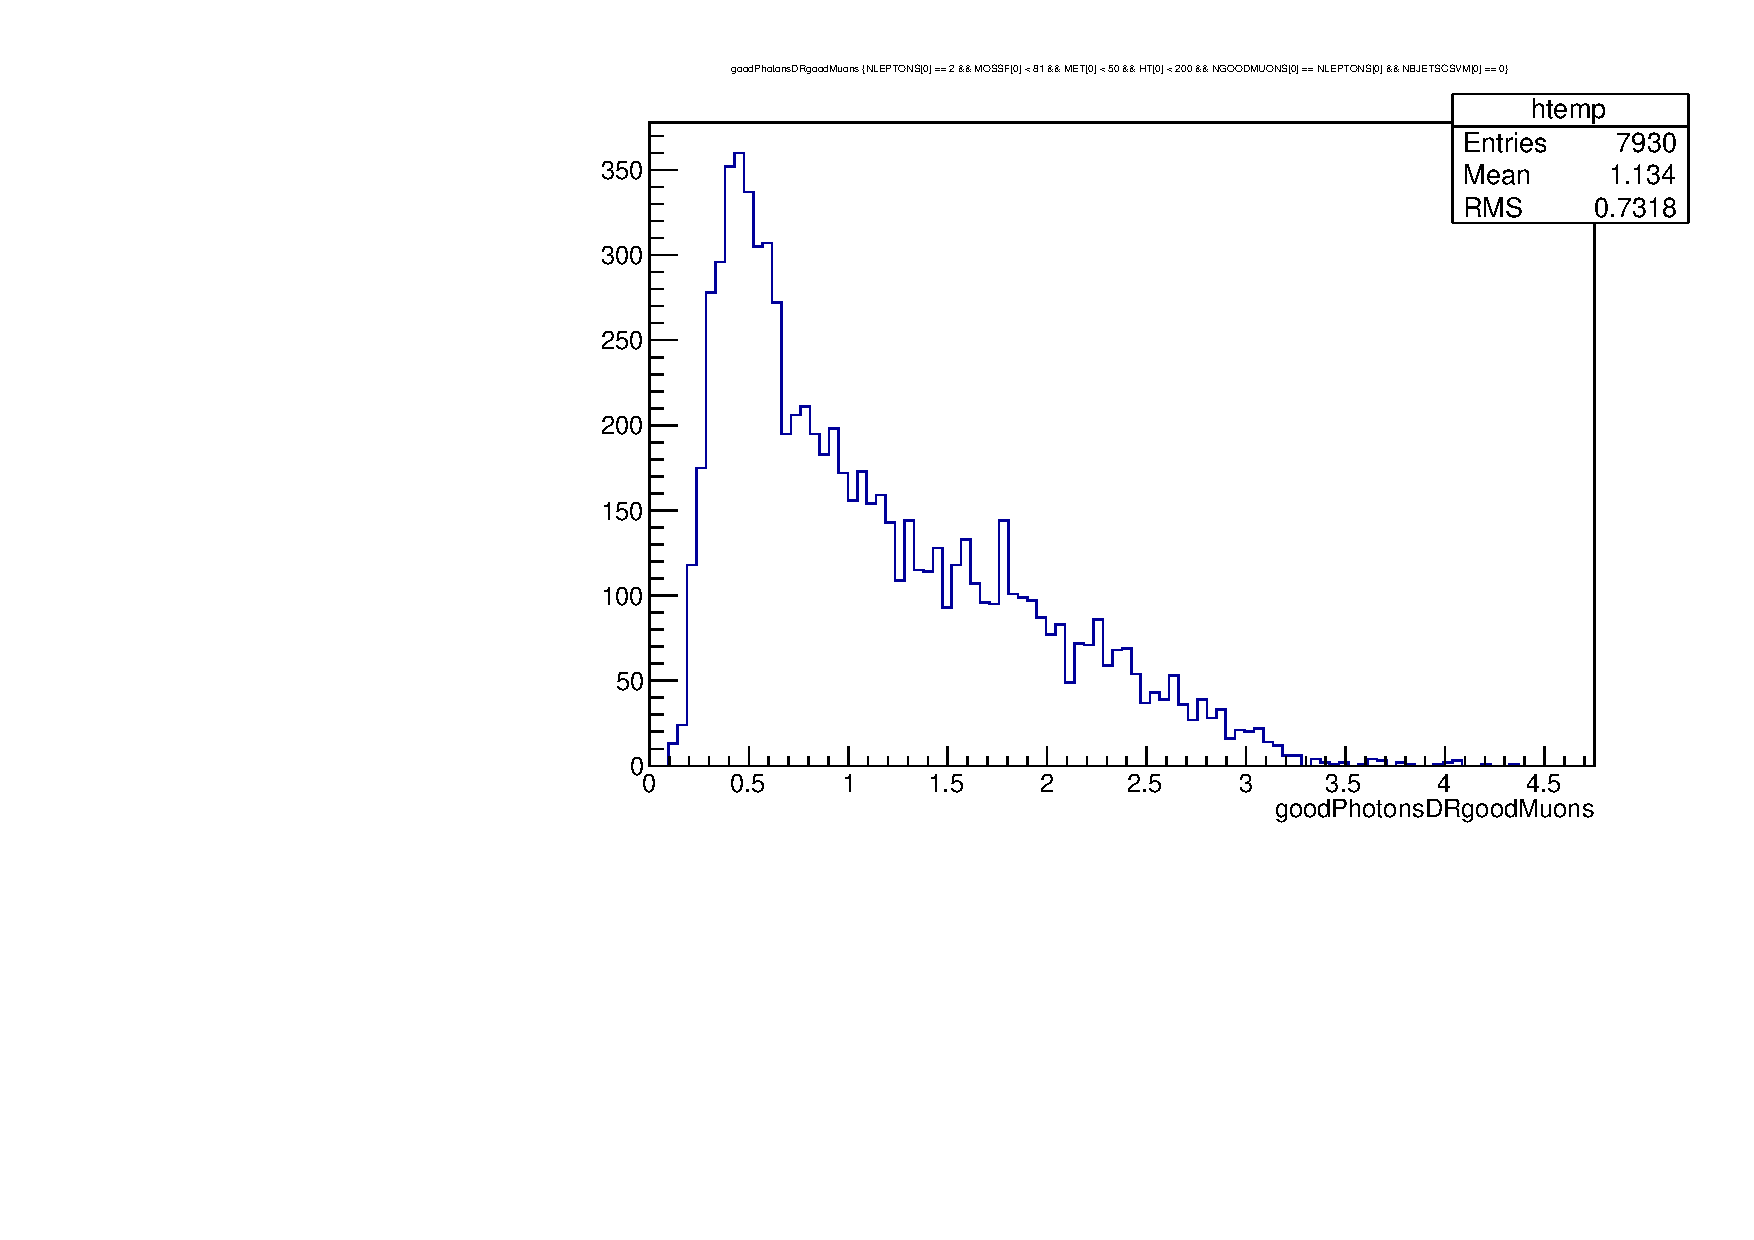
\includegraphics[width=\textwidth]{Background/bkg_fakeLight/goodPhotonsDRgoodMuons_AIC}
		\caption{AIC control region}
	\end{subfigure}
	\begin{subfigure}[b]{.7\textwidth}
		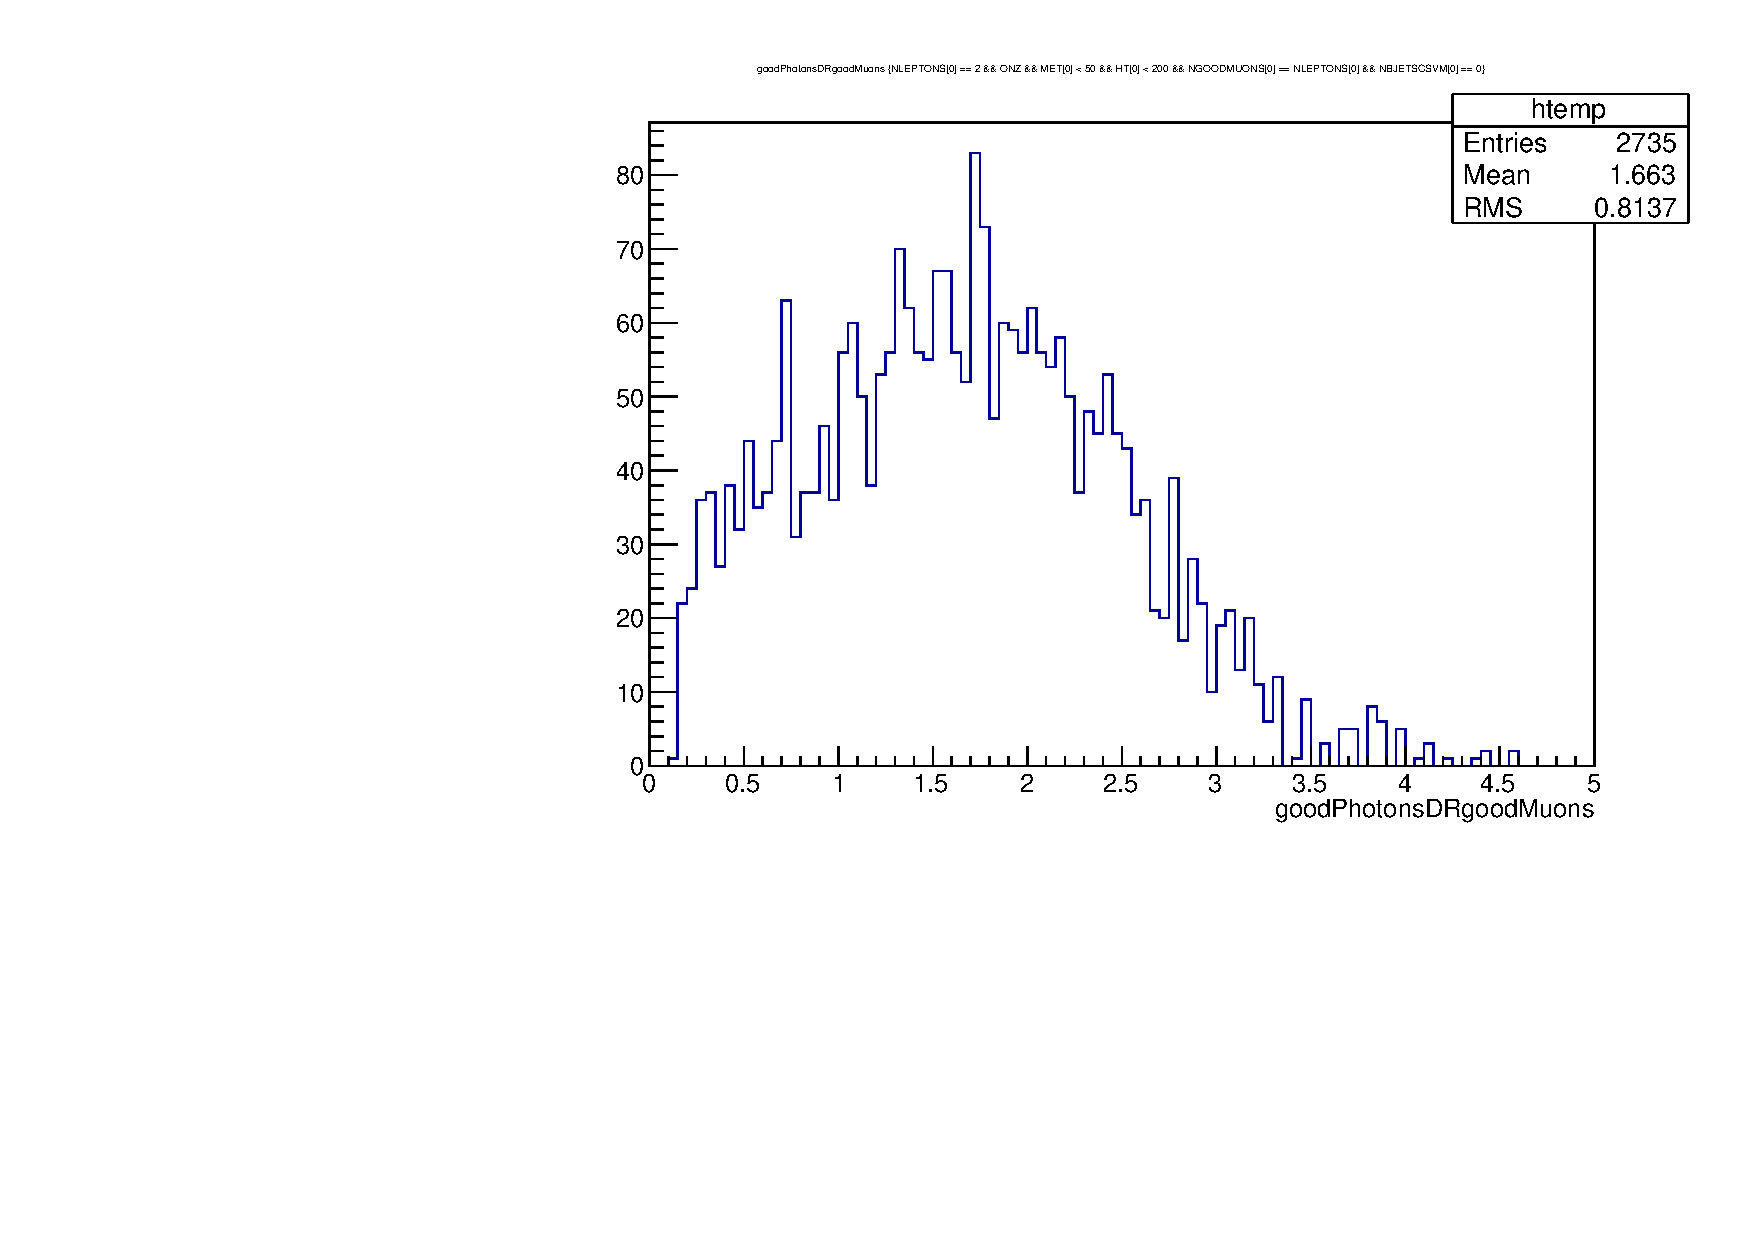
\includegraphics[width=\textwidth]{Background/bkg_fakeLight/goodPhotonsDRgoodMuons_ONZ}
		\caption{dilepton region on-\Z}
	\end{subfigure}
	\caption{$\Delta R$ distributions between photon and muon.
	\label{fig:fakeLight_AIC_DR}}
\end{center}
\end{figure}

Looking in the seed sample, we find that the $2\ell+\gamma$ mass indeed reproduces the \Z peak, as shown in Fig.~\ref{fig:fakeLight_AIC_MLEPTONS}. For photons faking muons, we find better shape agreement if we apply a loss factor of 0.8 to the photon \pt when creating the fake trilepton sample, attributing an average of 20\,\% of the \pt to the lost lepton. Outside the trilepton \Z window, it is necessary to increase the fake rate by 1.8 to achieve agreement.

\begin{figure}
\begin{center}
	\begin{subfigure}[b]{.7\textwidth}
		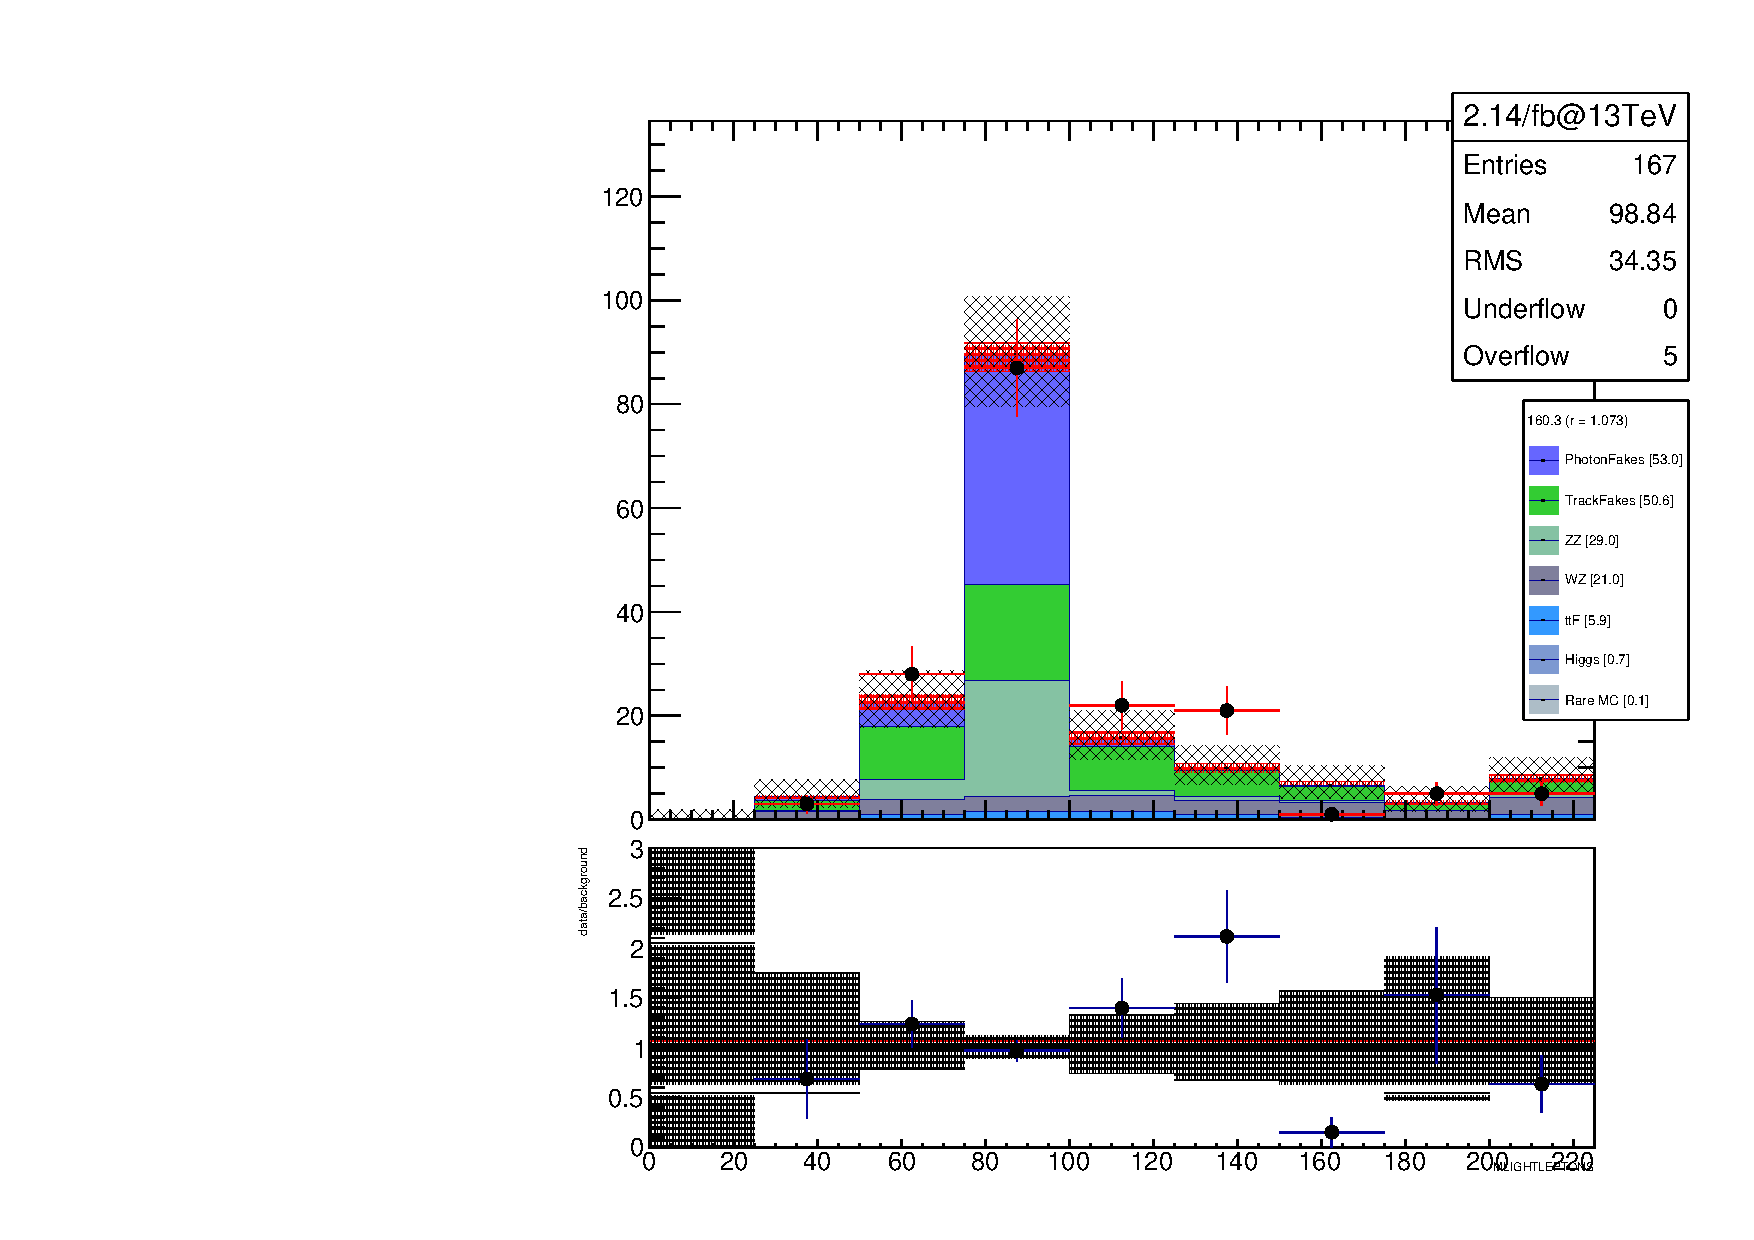
\includegraphics[width=\textwidth]{Background/bkg_fakeLight/AIC_MLIGHTLEPTONS_muFake}
		\caption{fake muon}
	\end{subfigure}
	\begin{subfigure}[b]{.7\textwidth}
		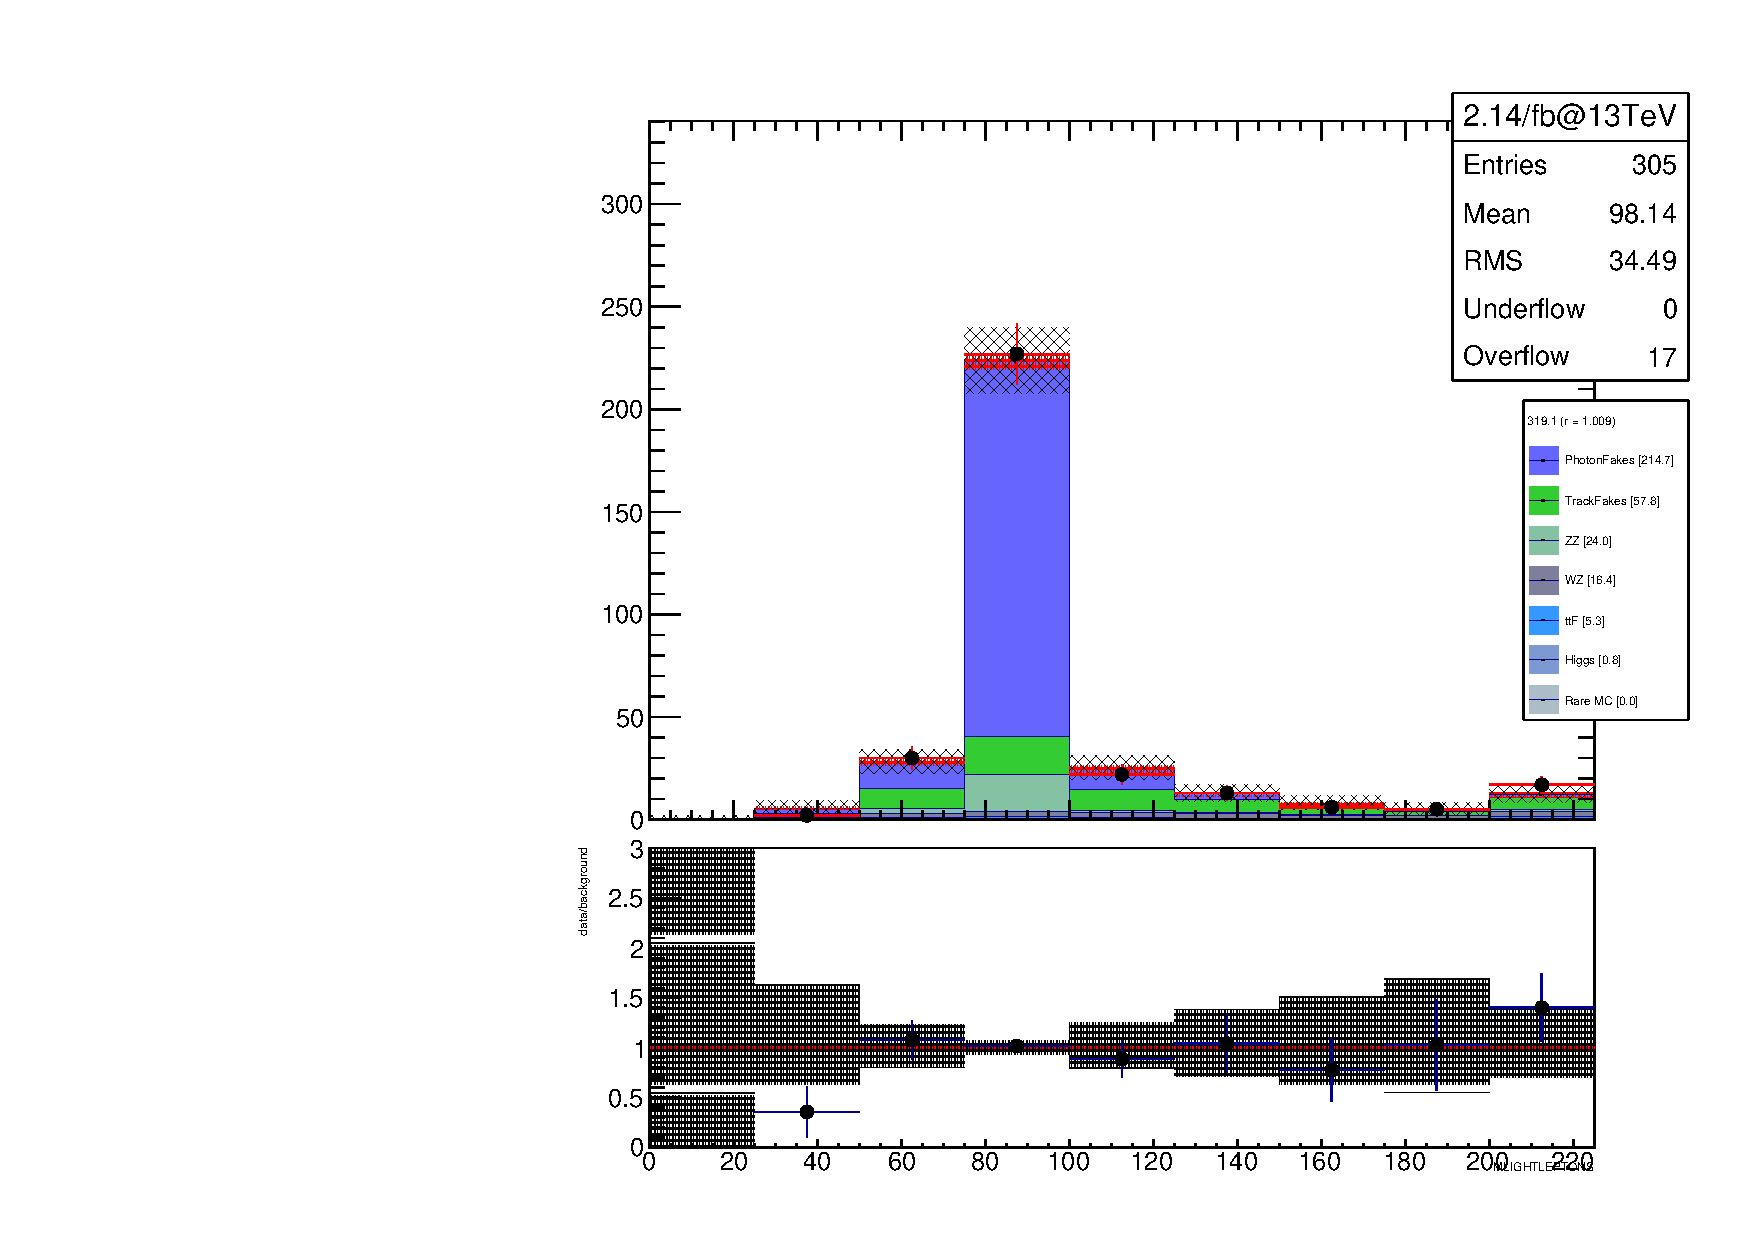
\includegraphics[width=\textwidth]{Background/bkg_fakeLight/AIC_MLIGHTLEPTONS_elFake}
		\caption{fake electron}
	\end{subfigure}
	\caption{$m_{3\ell}$ distribution in AIC-dominated control region.
	\label{fig:fakeLight_AIC_MLEPTONS}}
\end{center}
\end{figure}

After these corrections, we find that the photon fake rates are
\begin{itemize}
	\item muons: 1.60\,\% ($ee$ environment), 1.05\,\% ($\mu\mu$ environment),
	\item electrons: 3.5\,\% ($ee$ environment), 4.5\,\% ($\mu\mu$ environment).
\end{itemize}

We apply a 52\,\% systematic uncertainty on the total photon-based background estimate to cover the variation of observed fake rates as a function of the flavor of the remaining prompt lepton pair in the event.


\subsection{Fake Leptons from Jets}
In order to determine the background with fake electrons and muons from jets, we use isolated tracks a proxies. The isolation criteria that we require these tracks to satisfy are identical to our muon isolation criteria (see Sec.~\ref{sec:Selection/Object}). We produce a track-based fake 3$\ell$ background seed sample by reassigning isolated tracks to the lepton collections, so that the sample has one less lepton than the signal regions and an isolated track instead. All combinations are taken into account, \ie tracks are used to create both a fake-$e$ and a fake-$\mu$ event.\footnote{Multiple fakes in an event are not considered (neither of same proxy type (\eg two tracks) nor of different type). Hybrid fakes (one from a track, one from a photon) are currently not supported for technical reasons; same-type fakes however turned out to cause problems with the \ttbar MC subtraction. Given the smallness of the fake rates ($O(10^{-2})$), the contribution from multiple fakes is negligible anyways.} The fake background can then be estimated by applying the fake rate after requiring the signal region selection in this seed sample.

The fake rate $\frac{N(3\ell)}{N(2\ell + \textrm{track)}}$ is determined using events with 3 electrons or muons including an OSSF pair on-\Z and $\MET < 50\GeV$. This is the prominent \Z peak region with an additional lepton. As we subtract contributions from other backgrounds in the numerator and the denominator, this fake rate describes the number of fake leptons as a fraction of the number of 2$\ell$ + track events from all processes that are not modeled otherwise.

To achieve the best possible modeling, we make sure that the kinematic properties of the isolated tracks in this region resemble those of the fake leptons by applying weights to the track-based background in bins of the the lowest \pt lepton (proxy) which is generally the fake (Fig.~\ref{fig:fakeLight_Z_MINleptonPT}). Appendix~\ref{app:MOSSFlepton,track} contains additional plots supporting the suitability of tracks as lepton proxies. We then measure the number of 3$\ell$ events in data per 2$\ell$ + track event (fake rate), as a function of the flavor of both the fake lepton and of the \Z decay products and find:
\begin{itemize}
	\item muons: $(1.49 \pm 0.21)\,\%$ ($ee$ environment), $(1.49 \pm 0.17)\,\%$ ($\mu\mu$ environment),
	\item electrons: $(1.37 \pm 0.22)\,\%$ ($ee$ environment), $(1.75 \pm 0.19)\,\%$ ($\mu\mu$ environment).
\end{itemize}
Based on this, we use the electron and muon fake rates $(1.59 \pm 0.15\stat)\,\%$ and $(1.49 \pm 0.13\stat)\,\%$, respectively. We apply a systematic uncertainty of 14\,\% to cover the variation of observed fake rates as a function of the flavor of the remaining prompt lepton pair in the event.

To apply the fake rate in a signal region, we multiply it by the total number of events found in the corresponding 2$\ell$ + track region in data. However, since we use MC to obtain the fake contribution for the \ttbar background, we need to correct for double-counting. We thus subtract the contribution from 2$\ell$ + track events as predicted by the \ttbar MC from the data. To show that the subtraction is valid, we verify that the $n_\textrm{tracks}$ distribution in the \ttbar MC sample matches the one in data, so that we can trust the fake rate method used in data is applicable for the \ttbar MC subtraction (see Sec.~\ref{sec:bkg_tt}).

\begin{figure}
\begin{center}
	\begin{subfigure}[b]{.7\textwidth}
		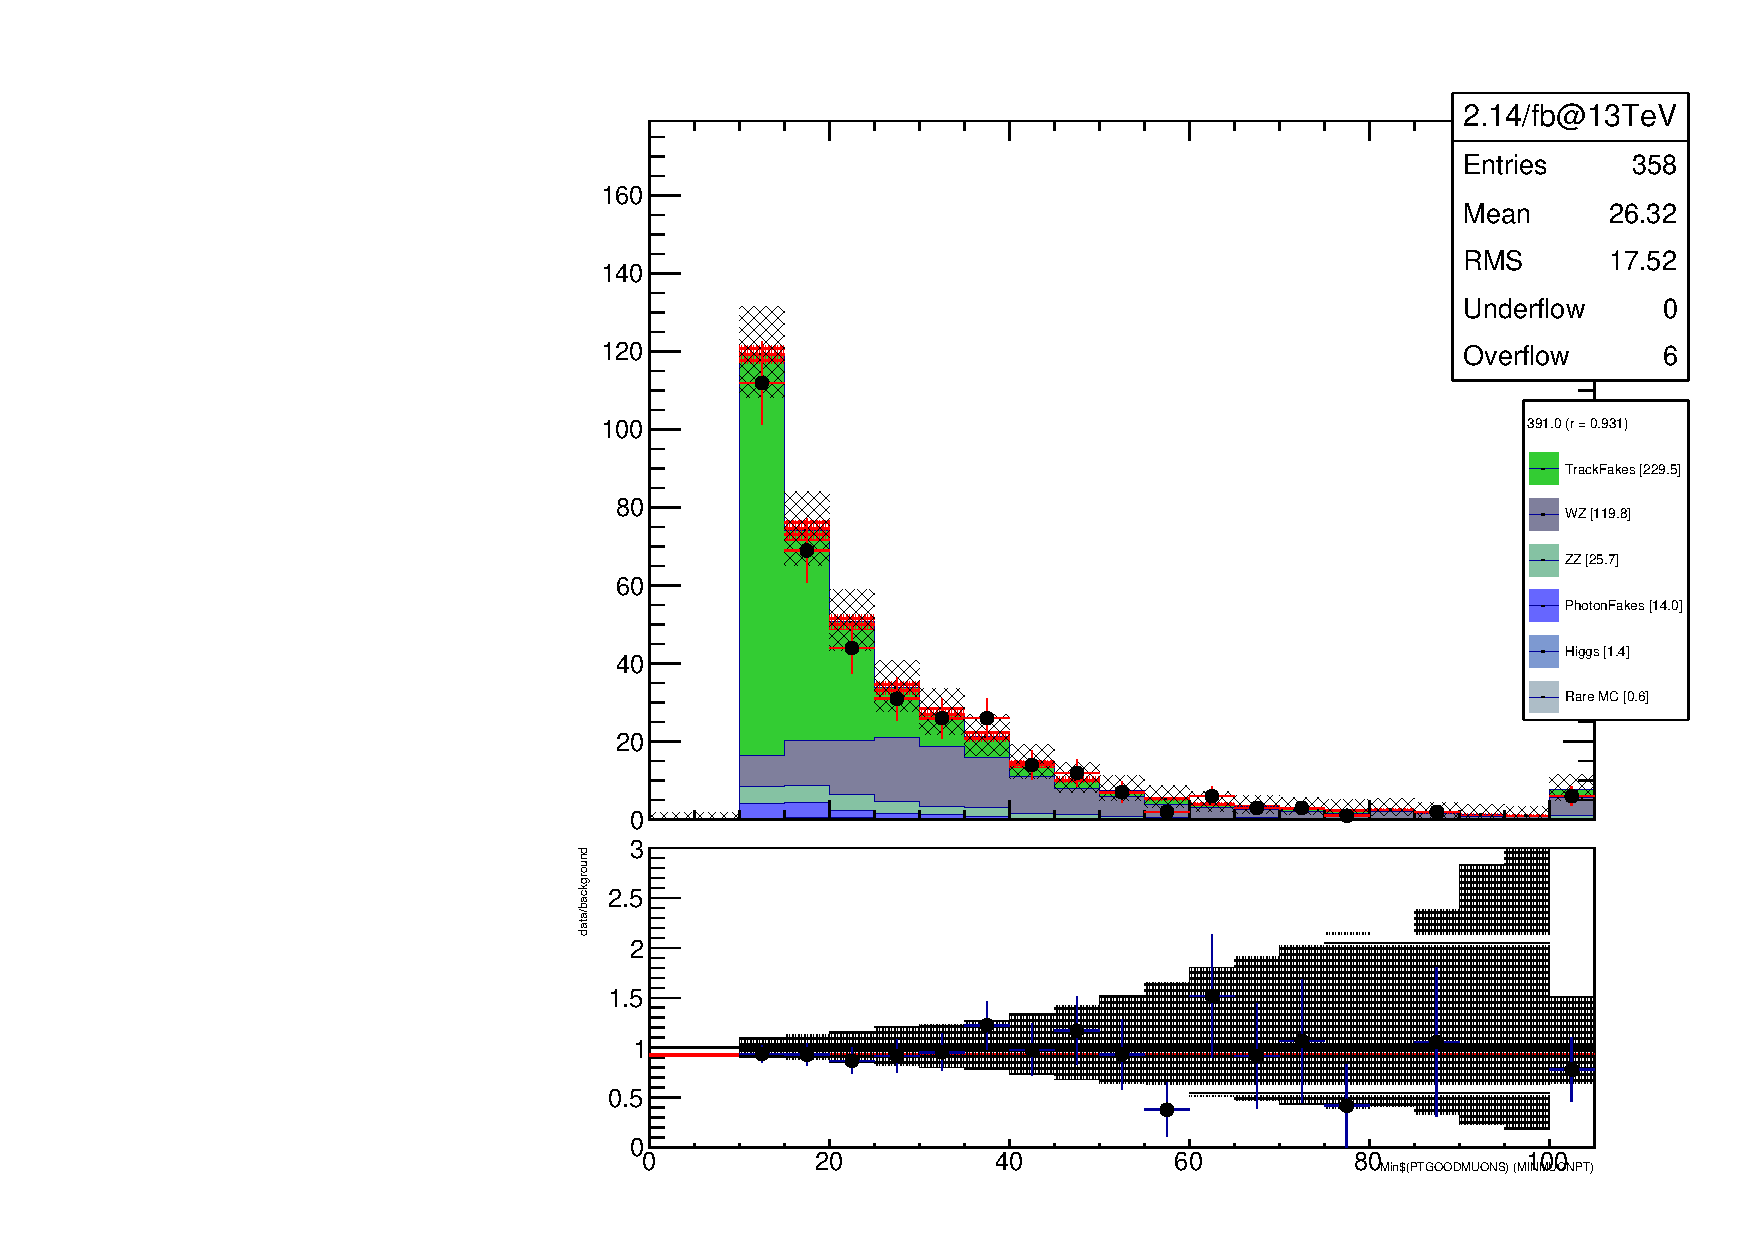
\includegraphics[width=\textwidth]{Background/bkg_fakeLight/Z_muFake_MINMUONPT}
		\caption{fake muon}
	\end{subfigure}
	\begin{subfigure}[b]{.7\textwidth}
		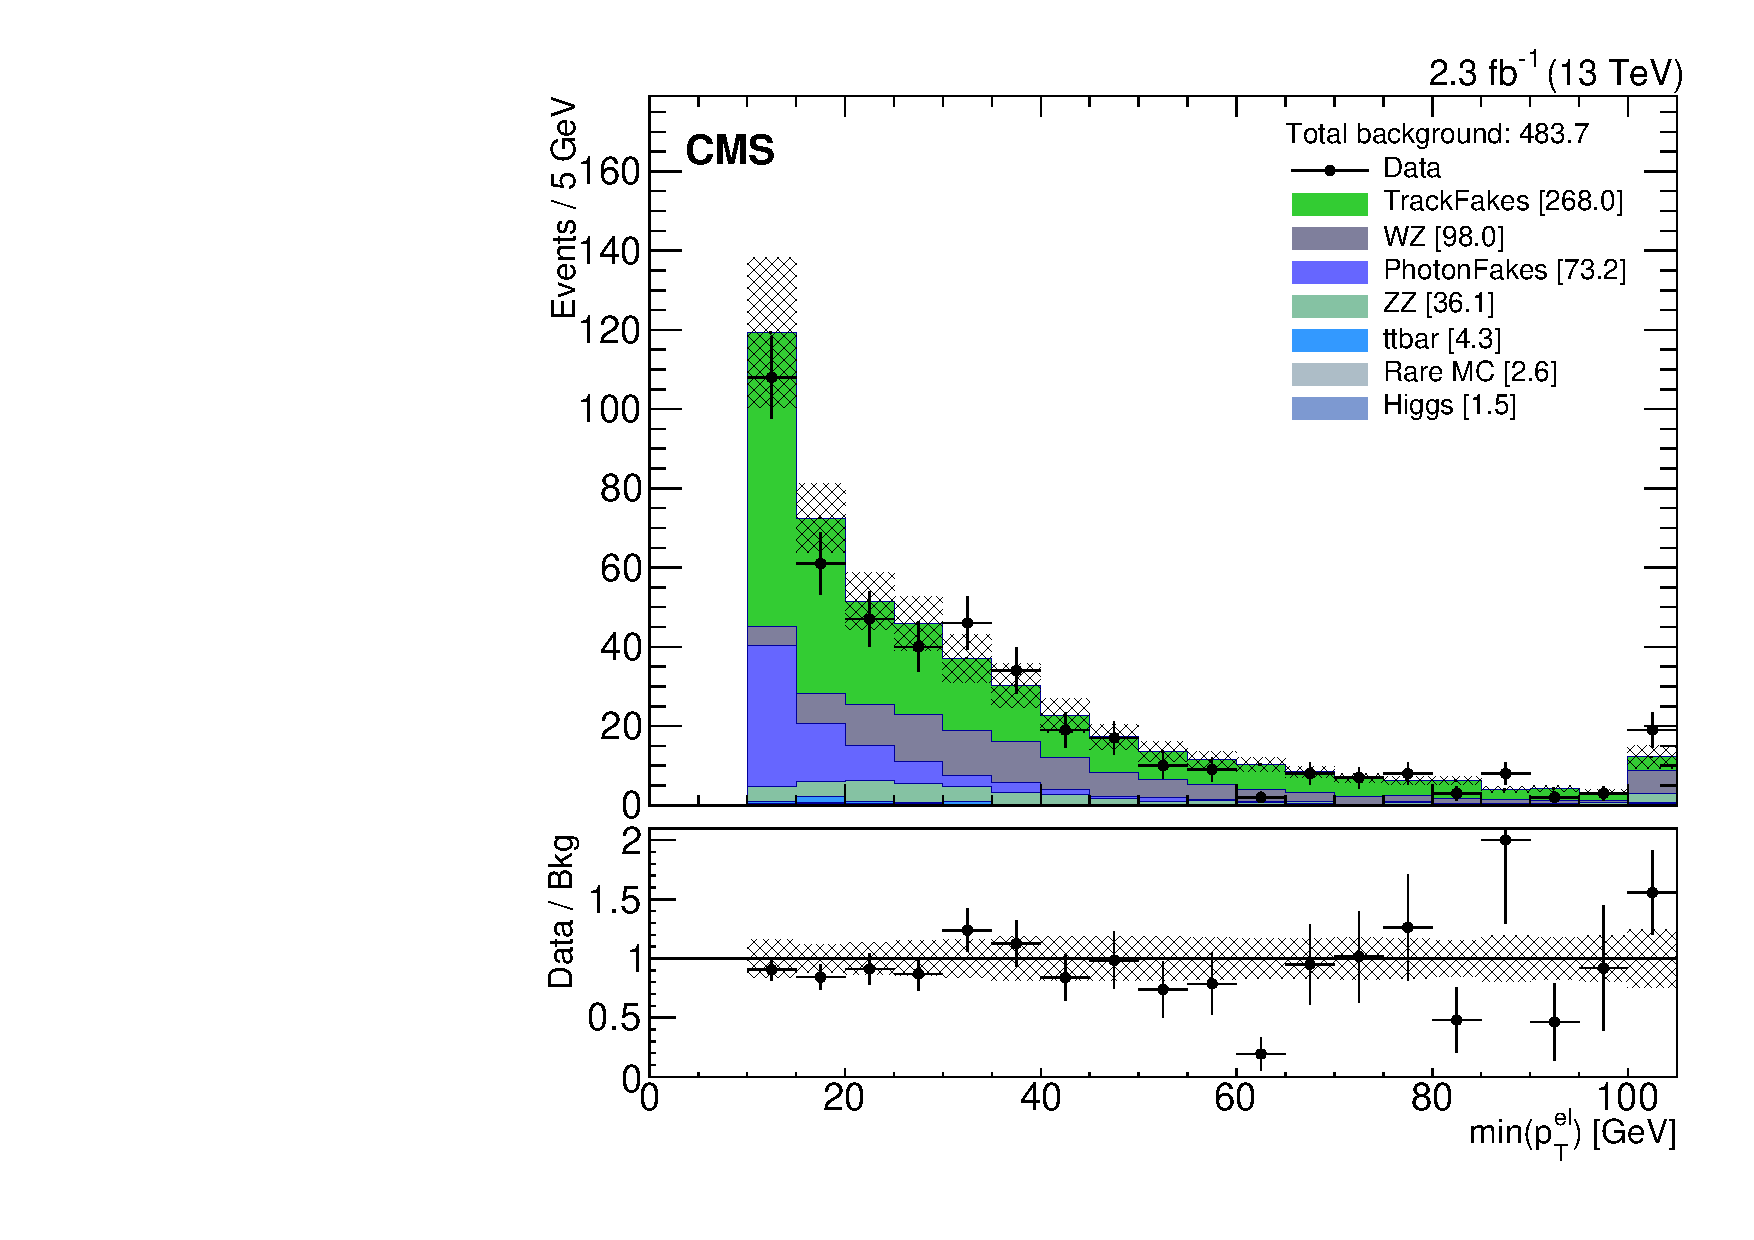
\includegraphics[width=\textwidth]{Background/bkg_fakeLight/Z_elFake_MINELECTRONPT}
		\caption{fake electron}
	\end{subfigure}
	\caption{\pt distributions of the lowest \pt lepton.
	\label{fig:fakeLight_Z_MINleptonPT}}
\end{center}
\end{figure}

Fig.~\ref{fig:fakeLight_Z_MOSSF} shows the mass distribution of the ``best'' OS dilepton pair across its full range in the trilepton control region, both with and without an AIC veto (for off-\Z events whose 3$\ell$ invariant mass is on \Z); Fig.~\ref{fig:fakeLight_Z_MOSSF_byFlavor} distinguishes by flavors. In case of ambiguity, the ``best'' OS dilepton pair is the one whose invariant mass is closest to the \Z mass, with the additional condition that pairs above the \Z window are not considered if there is a pair below the \Z window (thus shifting events from high-\Z to low-\Z, for a more separative background categorization, see Sec.~\ref{sec:Strategy/general}).

\begin{figure}
\begin{center}
	\begin{subfigure}[t]{.7\textwidth}
		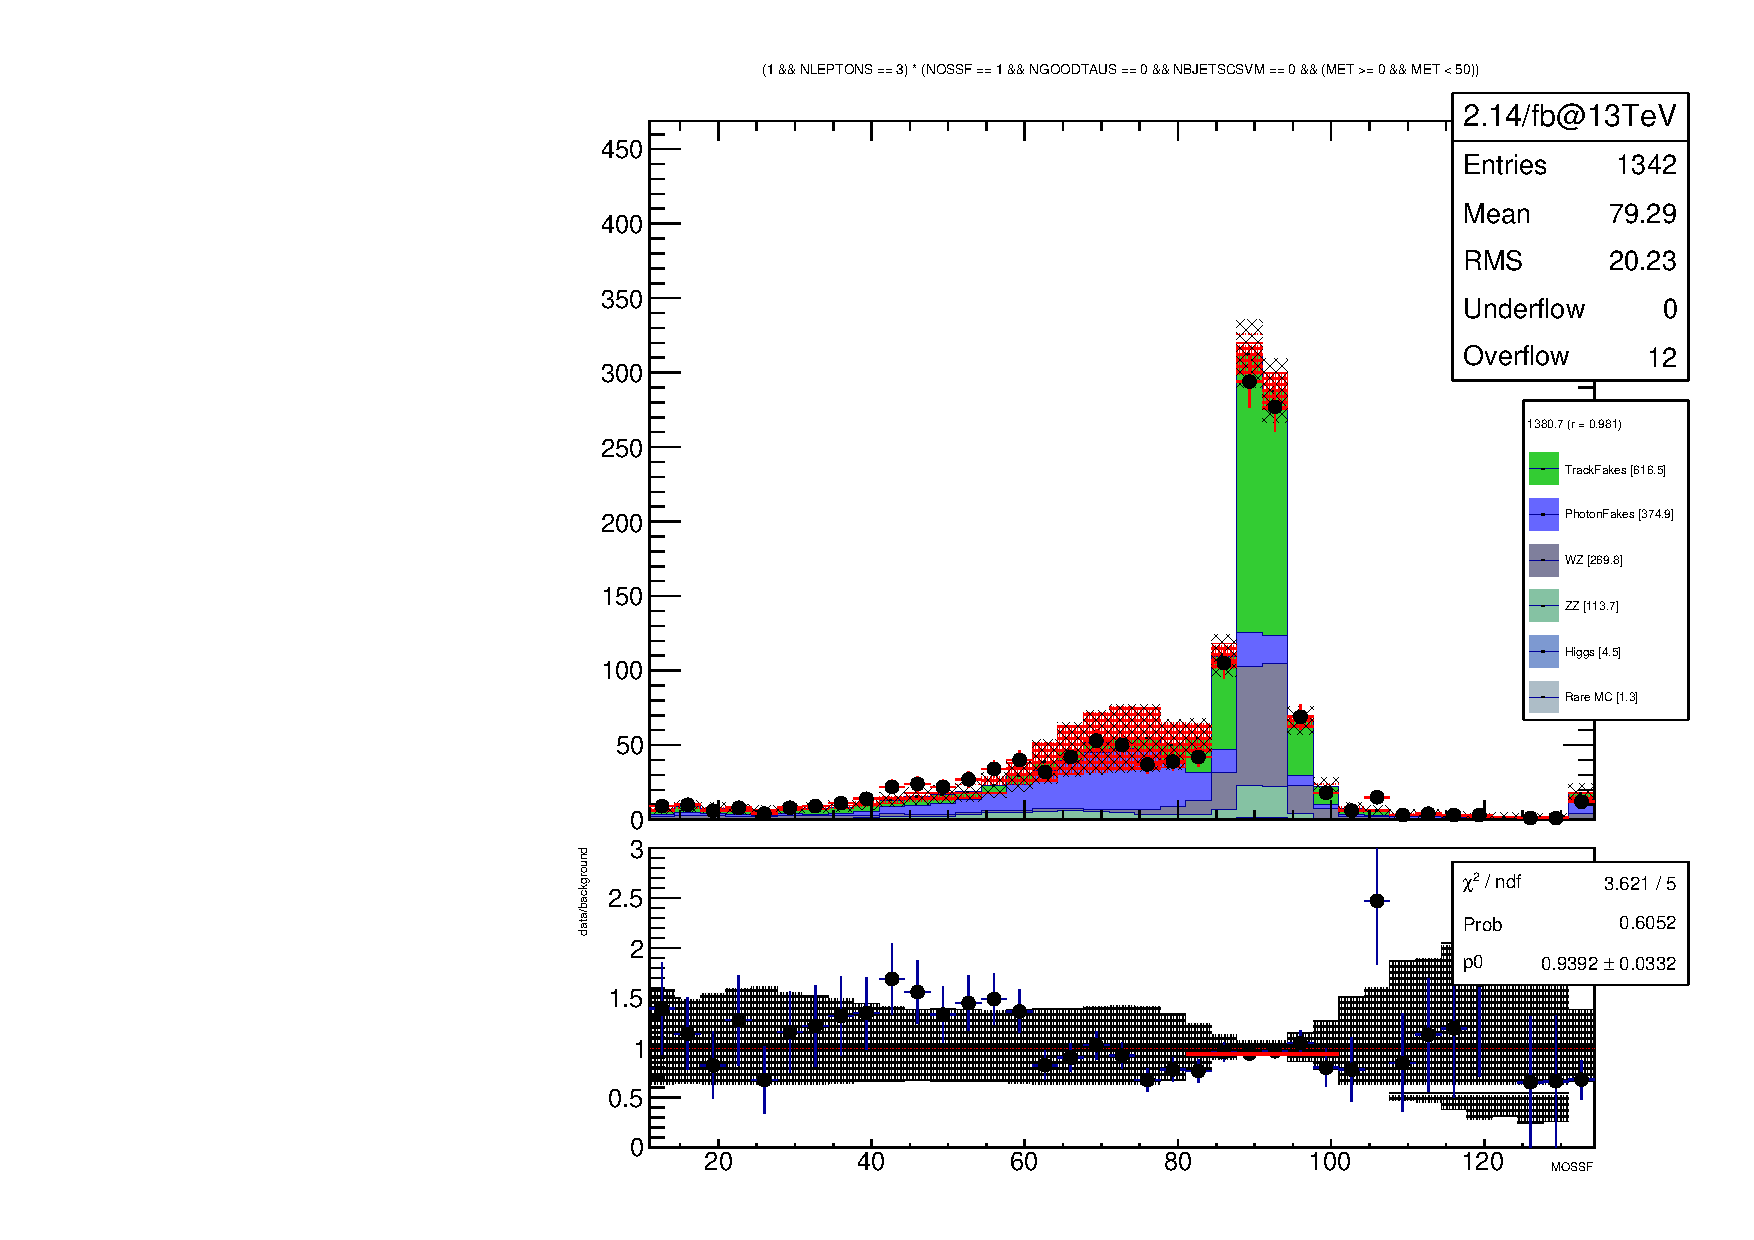
\includegraphics[width=\textwidth]{Background/bkg_fakeLight/Z_MOSSF}
		\caption{including events with $m_{\ell\ell\ell}$ on-\Z}
	\end{subfigure}
	\begin{subfigure}[t]{.7\textwidth}
		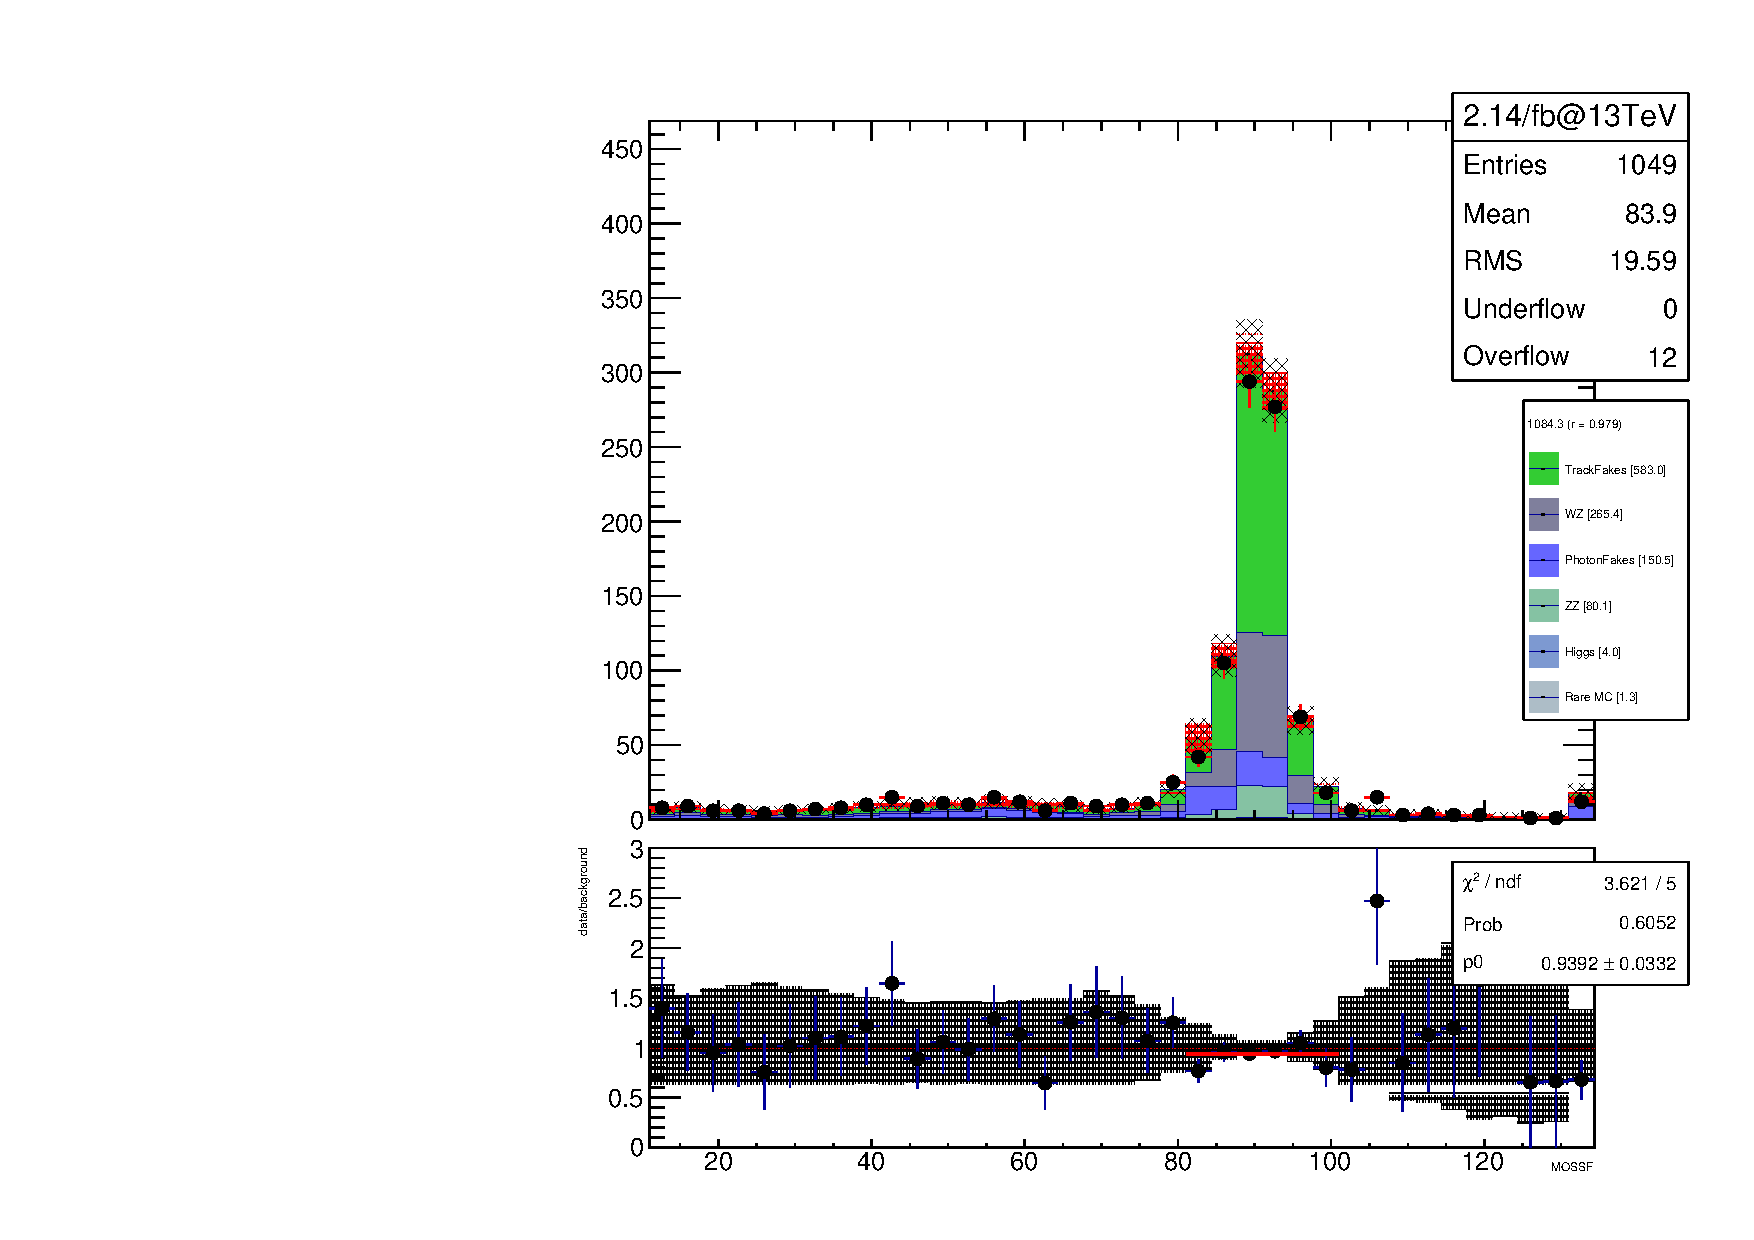
\includegraphics[width=\textwidth]{Background/bkg_fakeLight/Z_noAIC_MOSSF}
		\caption{events with $m_{\ell\ell\ell}$ on-\Z removed from the dilepton-off-\Z regions}
	\end{subfigure}
	\caption{$m_{\ell\ell}$ distribution in the dilepton + fake region.
	\label{fig:fakeLight_Z_MOSSF}}
\end{center}
\end{figure}

\begin{figure}
\begin{center}
	\begin{subfigure}[b]{.5\textwidth}
		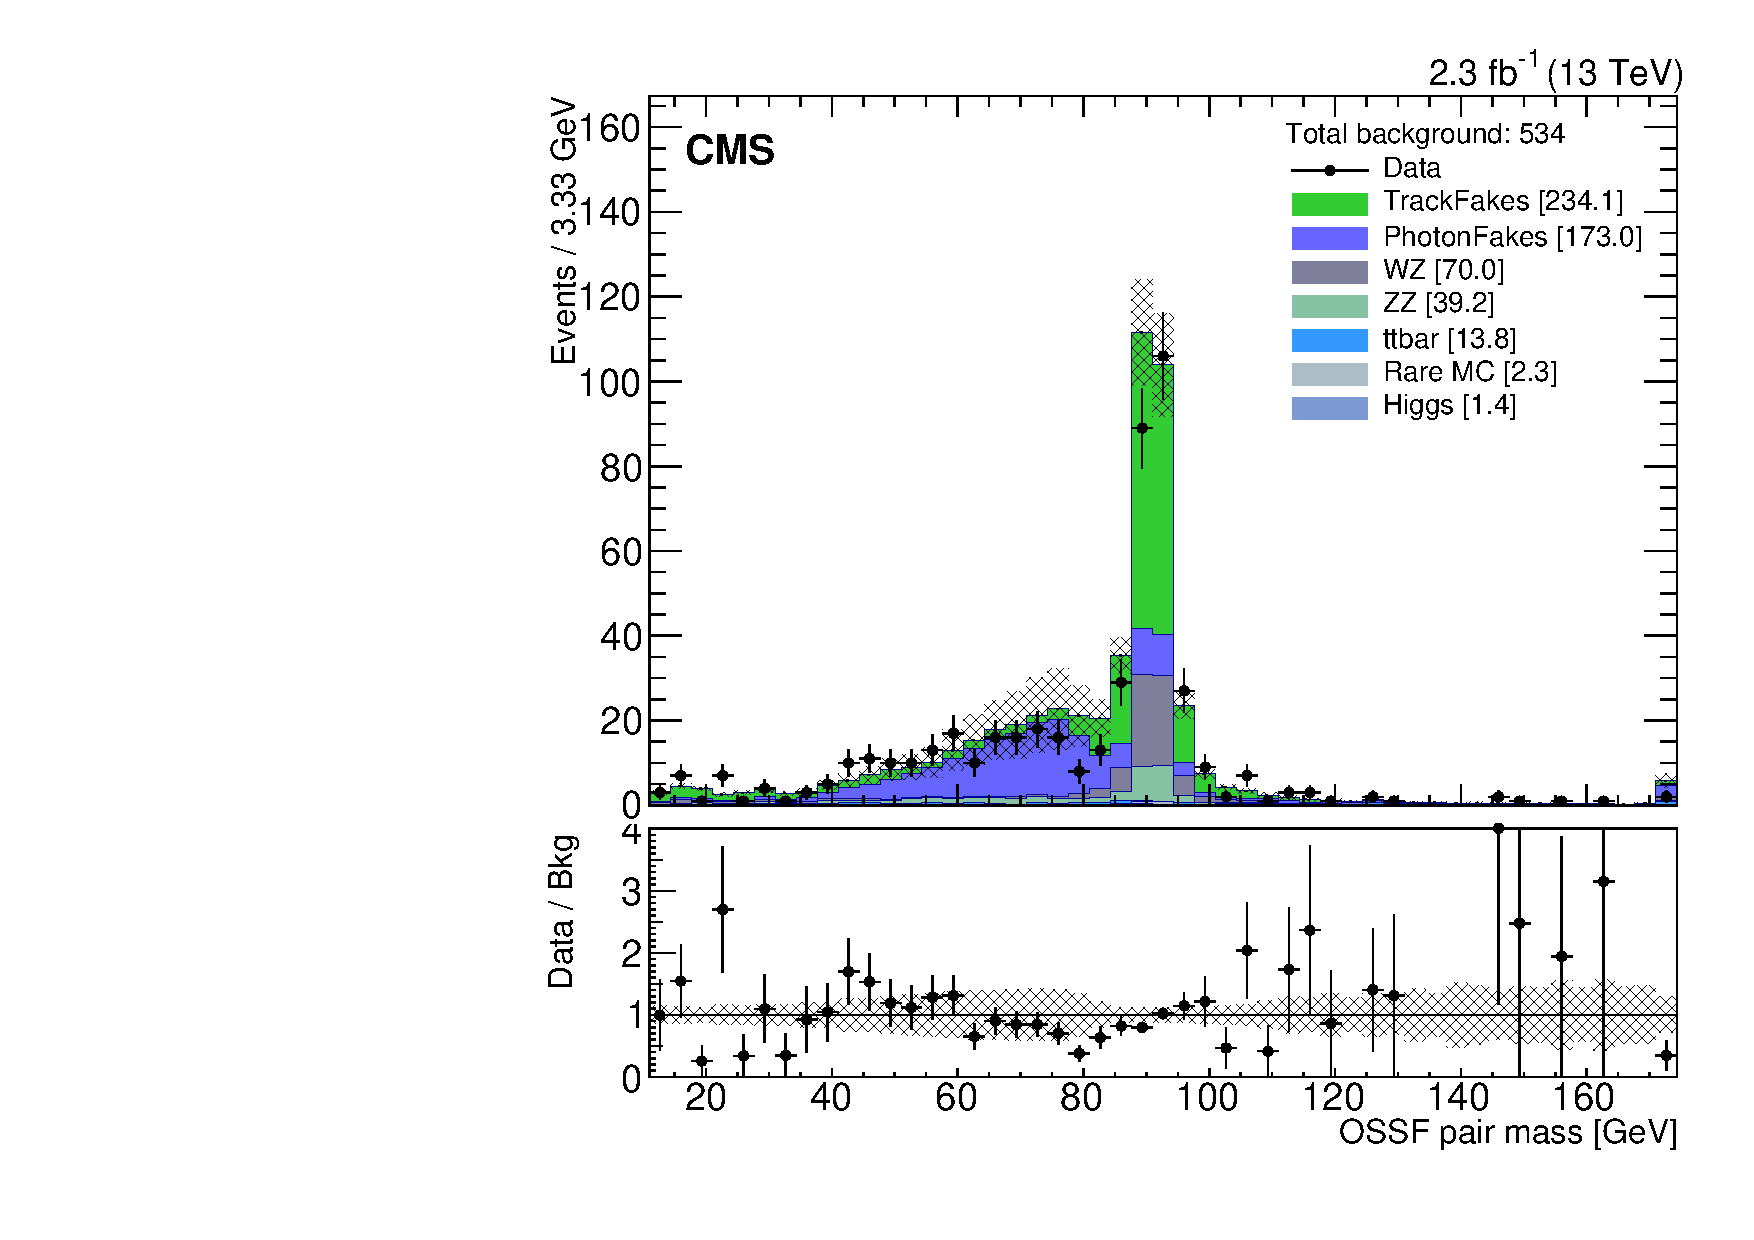
\includegraphics[width=\textwidth]{Background/bkg_fakeLight/Z_1el2mu_MOSSF}
		\caption{$e$ fake, $\Z \to \mu\mu$}
	\end{subfigure}%
	\begin{subfigure}[b]{.5\textwidth}
		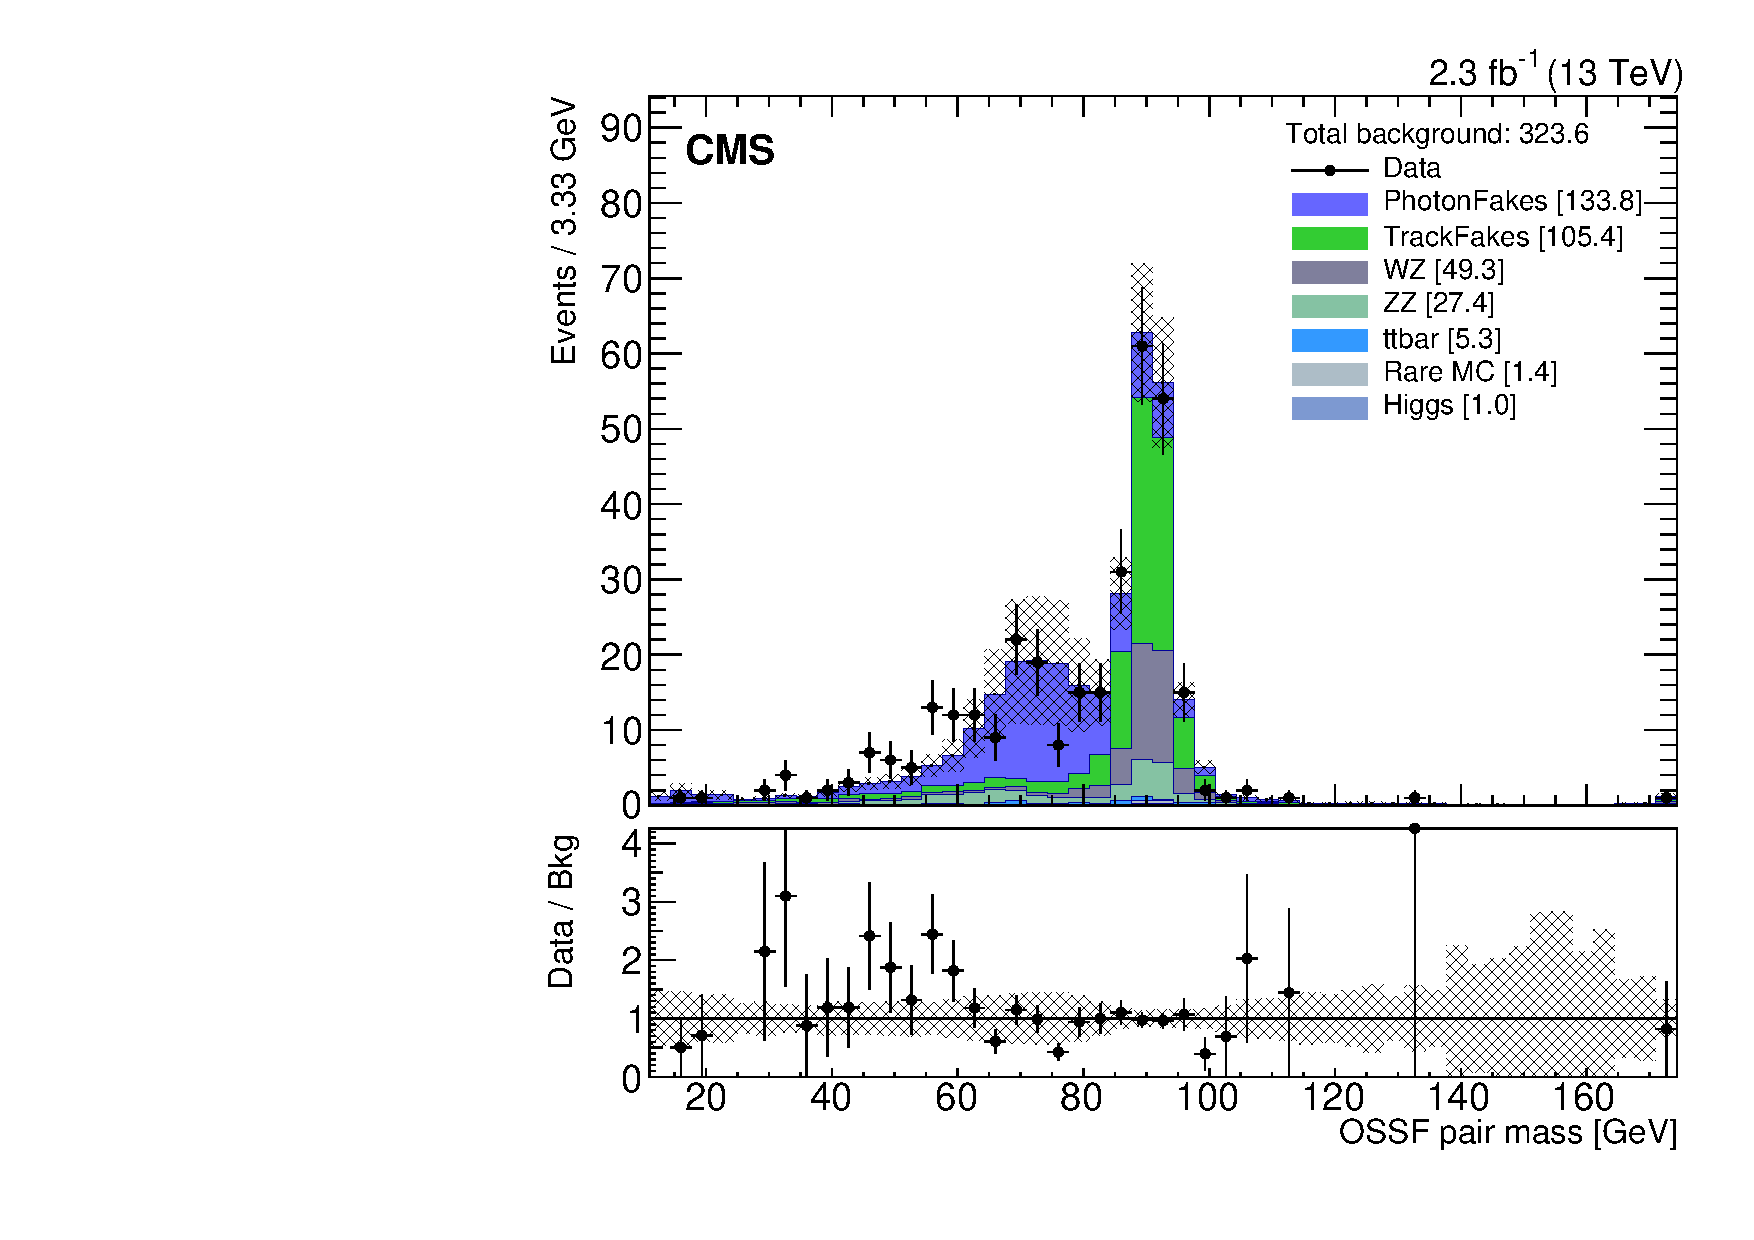
\includegraphics[width=\textwidth]{Background/bkg_fakeLight/Z_3el_MOSSF}
		\caption{$e$ fake, $\Z \to e e$}
	\end{subfigure}
	\begin{subfigure}[b]{.5\textwidth}
		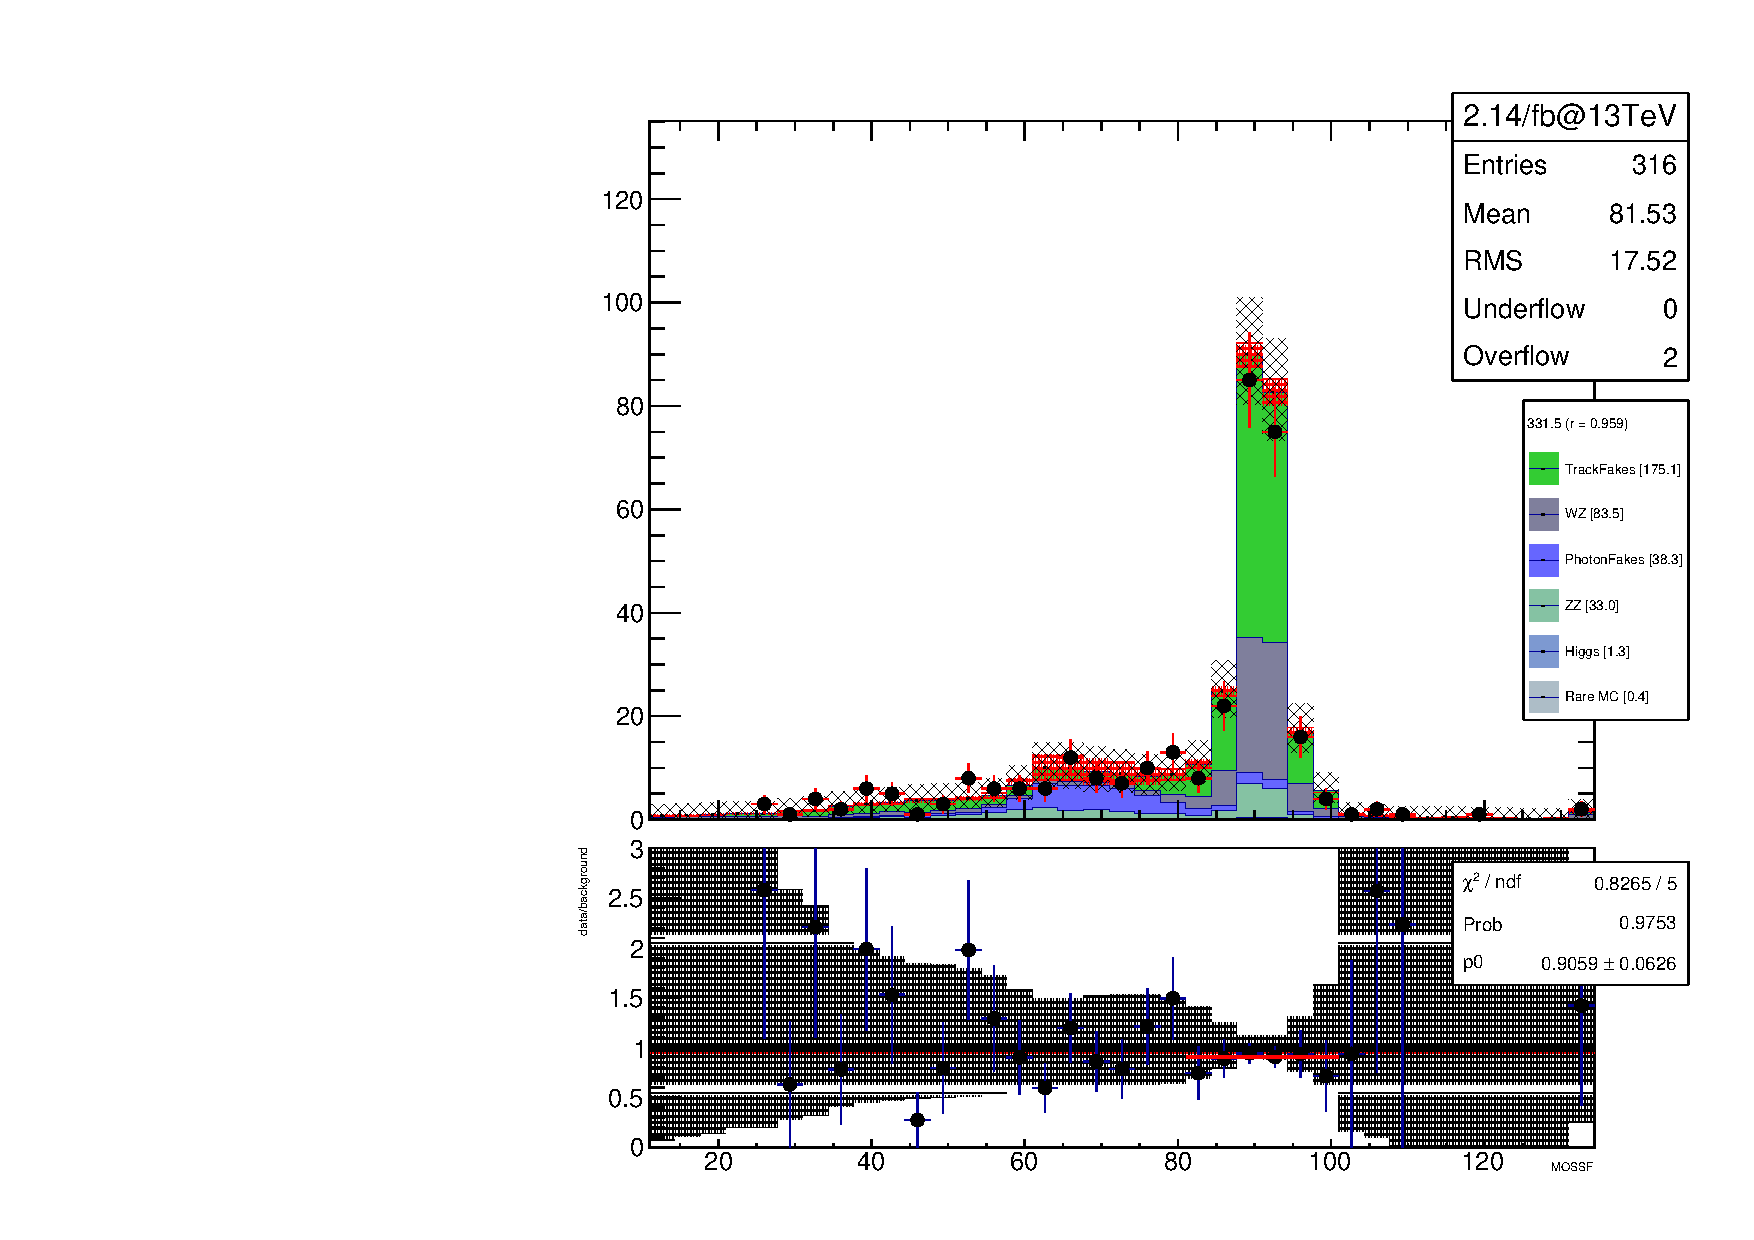
\includegraphics[width=\textwidth]{Background/bkg_fakeLight/Z_3mu_MOSSF}
		\caption{$\mu$ fake, $\Z \to \mu\mu$}
	\end{subfigure}%
	\begin{subfigure}[b]{.5\textwidth}
		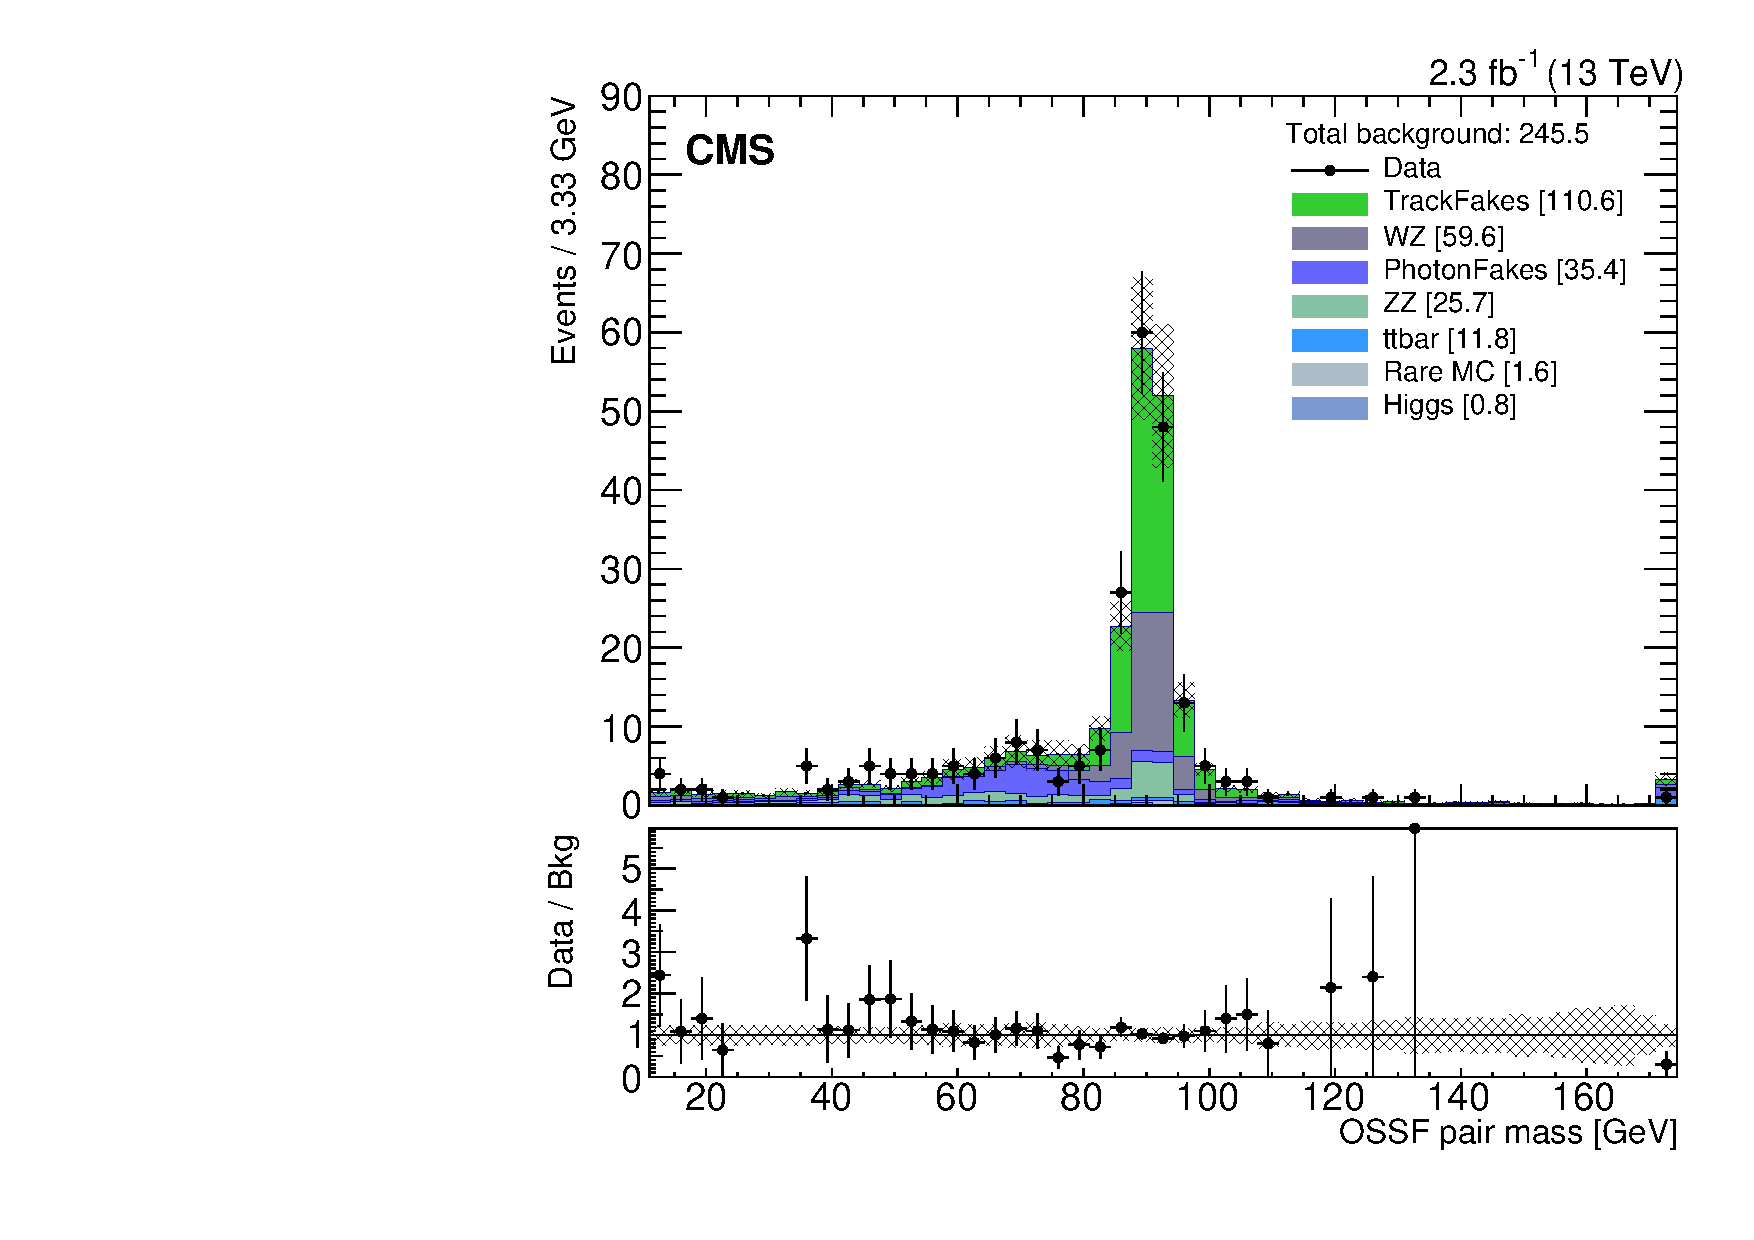
\includegraphics[width=\textwidth]{Background/bkg_fakeLight/Z_2el1mu_MOSSF}
		\caption{$\mu$ fake, $\Z \to e e$}
	\end{subfigure}%
	\caption{$m_{\ell\ell}$ distribution in the dilepton + fake region by flavor.
	\label{fig:fakeLight_Z_MOSSF_byFlavor}}
\end{center}
\end{figure}

As an additional cross-check, we show the \HT distribution in the \Z region (Fig.~\ref{fig:fakeLight_Z_HT}).
\begin{figure}
\begin{center}
	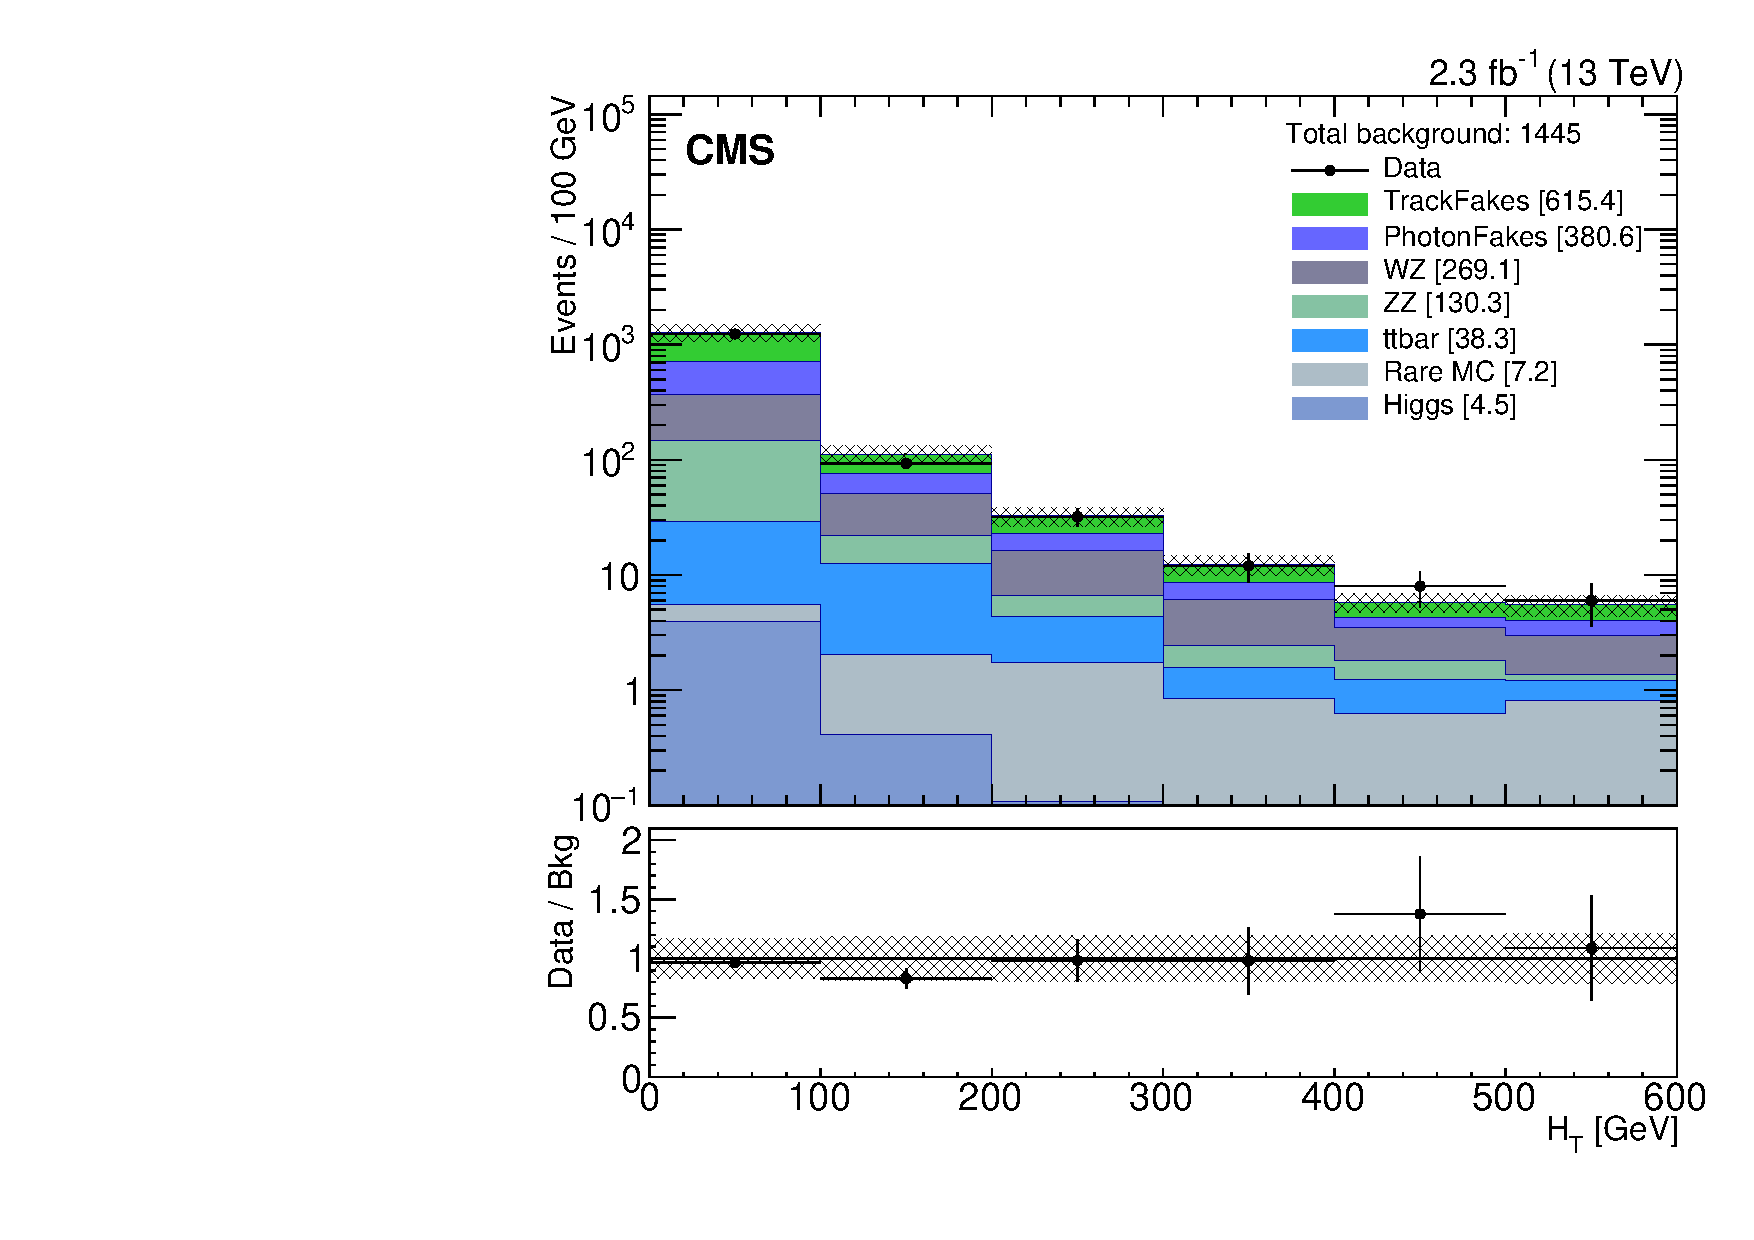
\includegraphics[width=.7\textwidth]{Background/bkg_fakeLight/Z_HT}
	\caption{$\HT$ distribution in the dilepton fake region (no OSSF pair mass cut).
	\label{fig:fakeLight_Z_HT}}
\end{center}
\end{figure}
Finally, we perform a closure test in Drell-Yan MC, comparing the on-Z and off-Z behavior in the control trilepton region (see Fig.~\ref{fig:fakeLight_closure}). We find that the fake rates agree within 5\,\% on and off Z. The statistical uncertainty of the numerator in the high-Z region is 15\,\%.

\begin{figure}
\begin{center}
	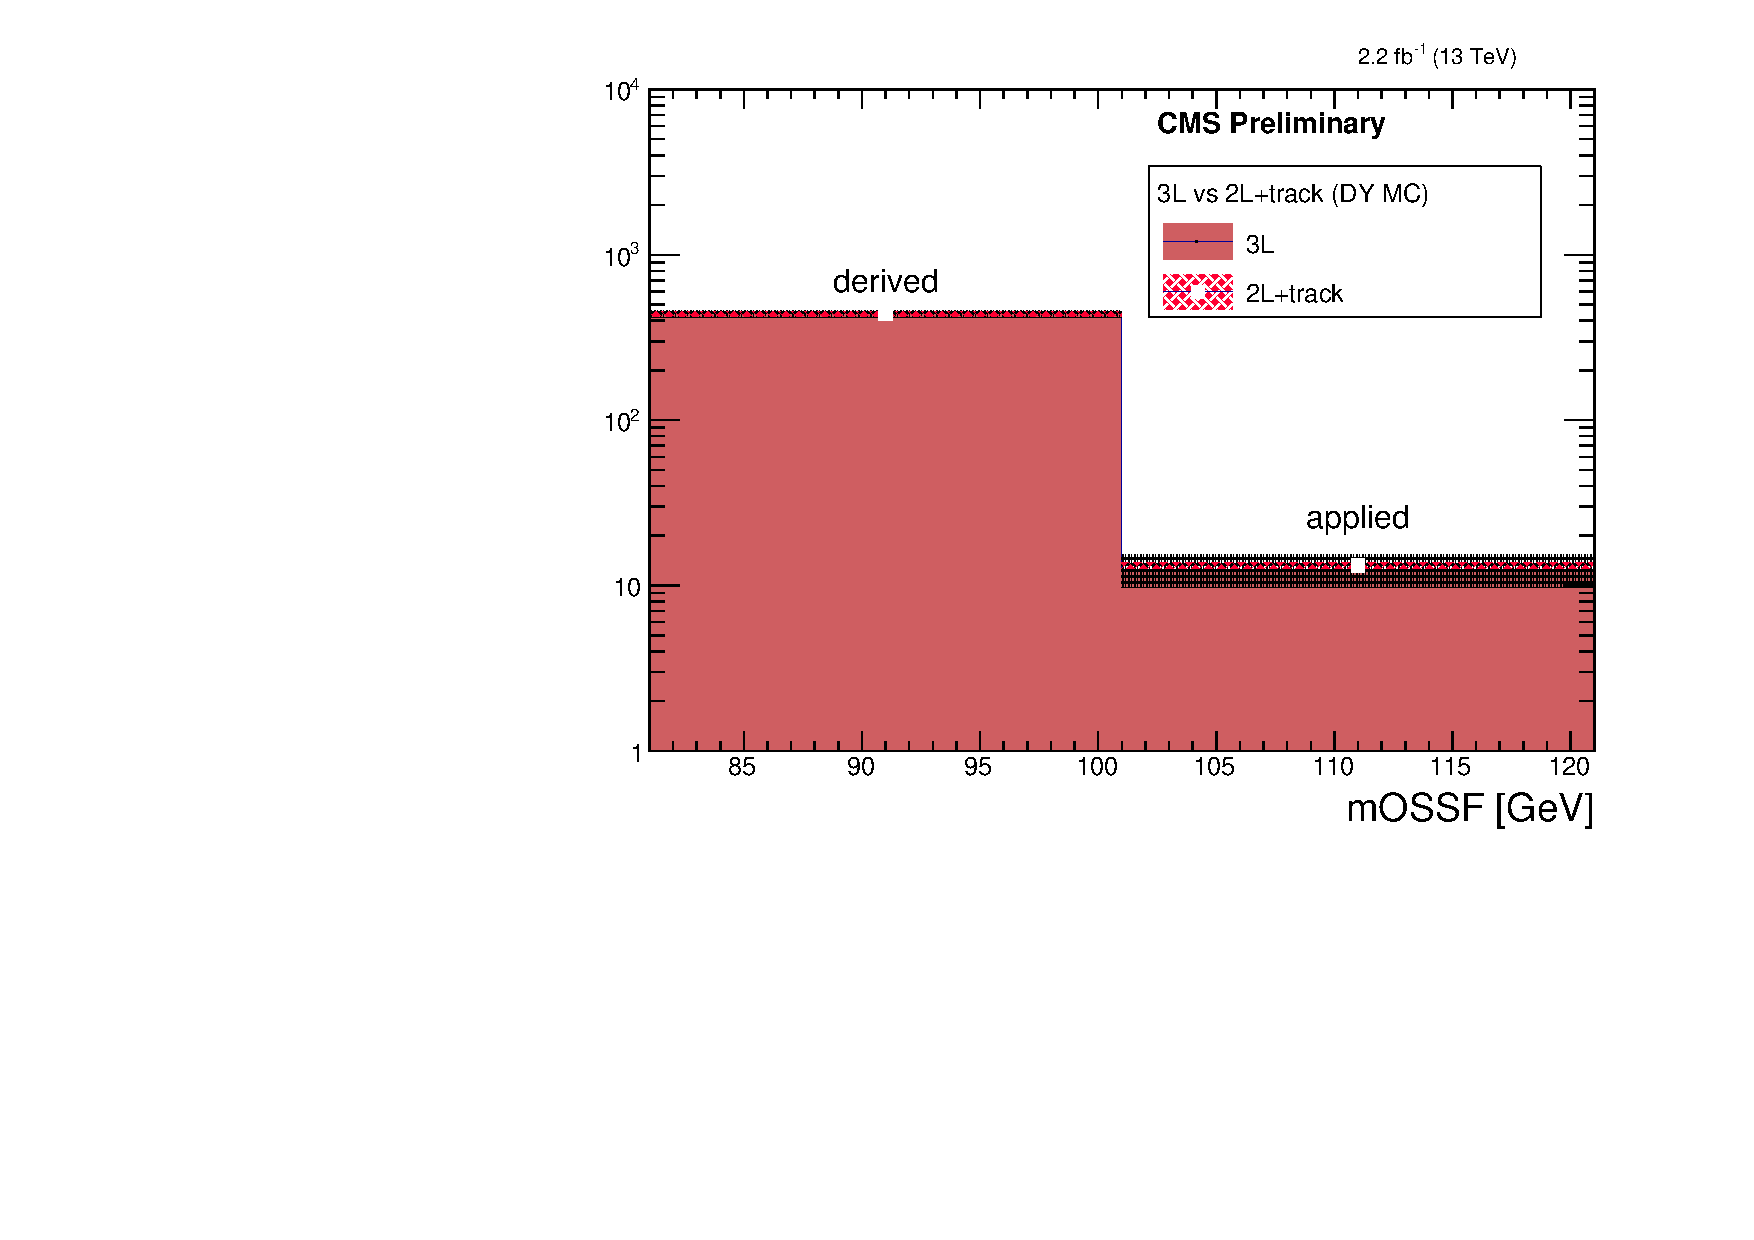
\includegraphics[width=.7\textwidth]{Background/bkg_fakeLight/L3vsL2T1_MOSSF-formatted}
	\caption{Closure test in Drell-Yan MC for the track-based fake rate method. The plot compares the 3-lepton yield with the prediction from 2 leptons + track proxy. The second bin in this plot ranges from 101 GeV to infinity.
	\label{fig:fakeLight_closure}}
\end{center}
\end{figure}
